\cotefile{10}
\scanpage{131}

b) Exemple d'un $\otimes$ foncteur exact fidèle, compatible avec $\deleted{\unsure{k\handwritten{\varphi}|k\handwritten{\psi}}}$ $1,\handwritten{\unsure{\varphi|\phi}},{}^{\handwritten{\unsure{\vee|\nu|v}}}$ (mais pas \deleted{avec} $\handwritten{\unsure{\psi|\varphi|\mu}}$ !), et qui n'est pas localement isomorphe au foncteur fibre donné. - On prend pour $G$ un groupe. On note alors que la donnée d'un système de $\deleted{W}\handwritten{L}_{g}$ et d'isomorphismes $(*)$ \deleted{avec $(**)$}, satisfaisant les diverses compatibilités, est équivalente à la donnée d'une extension de $G$ par $k^{\handwritten{*}}$. Le foncteur $\inserted{F'}$ est isomorphe \unsure{au|ay} foncteur $F$ sss cette extension splitte. L'ensemble des classes d'isomorphie de foncteurs fibres définis sur $k$ est ainsi en correspondance 1-1 avec $H^{2}(G,k^{\handwritten{*}})$. Or Même si $G$ est commutatif (par exemple le produit de deux groupes cycliques isomorphes d'ordre premier à \deleted{$k^{\handwritten{*}}$) et $k$} $\mathrm{car}.k$) et $k$ algébriquement clos, le $H^{2}$ peut être non nul; \deleted{\unsure{il ne se tue alors dans}} d'ailleurs un élément non nul de $H^{2}$ ne se tue dans aucune extension de $k$ (si $k$ alg. clos), d'après le principe de l'\unsure{extension|extensiion} finie.

Si cependant $G$ est commutatif, et si on se borne aux $F'$ compatibles avec $\handwritten{\psi}$ également, on trouve les extensions commutatives de $G$ par $k^{\handwritten{*}}$; si $k$ est algébriquement clos, donc $k^{\handwritten{*}}$ divisible, alors toute telle extension splitte, donc $F'$ est alors isomorphe à $F$ (en \unsure{confôrmité|conformité} avec la théorie galoisienne relative au cas où l'application diagonale de $U$ est commutative ...).

Ainsi, il peut y avoir des foncteurs fibres compatibles avec $\handwritten{\psi}$ donné, et d'autres qui ne le sont pas et qui par suite ne sont pas loc. isom. au premier. Cela montre donc \margin{\handwritten{\unsure{étudier} les contraintes de comm. \unsure{+|\&} \unsure{associon|assoc.} \unsure{aux graduations|des graduations} mod 2.}} \unsure{qu'on|qu'ôn} ne peut négliger la \deleted{condition de} contrainte de commutativité comme on aurait aimé pouvoir le faire. De plus, \margin{\figure{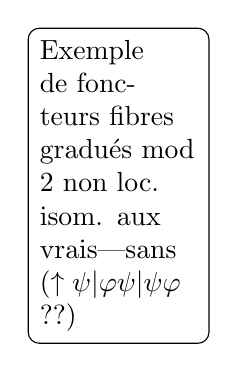
\begin{tikzpicture}
\node[text width=2cm,inner sep=4pt] (n) {\handwritten{Exemple de foncteurs fibres \unsure{gradués} mod 2 non loc. isom. aux \unsure{vrais|sans} $(\unsure{\uparrow\psi|\varphi\psi|\psi\varphi}$ ??)}};
\draw[rounded corners] (n.north west) -- (n.north east) -- (n.east) -- (n.south east) -- (n.south west) -- cycle;
\end{tikzpicture}}} cela suggère qu'en l'absence de contrainte de commutativité, la classification des foncteurs fibres se fait par des groupes du type de cohomologie de Brauer.

% archive sheet number: 130
